\documentclass[11pt]{scrartcl}
\usepackage[T1]{fontenc}
\usepackage[utf8]{inputenc}

\title{COS10004 Computer Systems Assignment 1}
\author{Daniel Coady (102084174) -- 12:30 Wednesday}
\date{19/09/2019}

\usepackage{graphicx}
\usepackage{fancyhdr}
\pagestyle{fancy}
\lhead{Daniel Coady (102084174)}
\rhead{COS10004 Computer Systems -- Assignment 1}

\begin{document}

\maketitle

\pagebreak

\section*{Stage 1}
\begin{figure}[h]
    \centering
    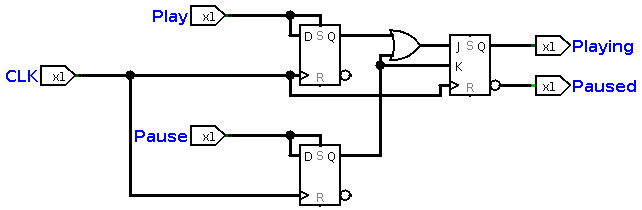
\includegraphics[scale=0.5]{images/stageone.png}
    \caption{Circuit used for stage one -- Play/pause functionality}
\end{figure}
For this stage I have two inputs for play and pause. The way this is structured is by having
a sort of latch for each input so that on a button press the state is stored for the next
clock cycle to act upon. The latch is very simple, consisting of a D flip-flop that has both
the set and D pins connected to the button. This is so that as soon as the button is pressed
it's state is set and stored until the next clock cycle. It's important to note as well that
the D pin must be connected to the button along with the set pin. This is because without
doing so the latch would not be able to ever reset back to a 0 state, making it not very useful.
Once we pass the latch, the play button goes into the J input of a JK flip-flop which turns
on the Q output for us. The play button is similar in that it then feeds into the K input of
the JK flip-flop, however we also need to give the pause button the ability to start playing
again from a paused state if pressed. To do this we can connect the pause button to both J and
K inputs, transforming it's functionality into a T flip-flop when the pause button is pressed.
There is one issue however: the play button is already connected to the J input to trigger the
playing state. To get around this so that we can allow both the play and pause buttons use the
J input we can use an or gate which both buttons will connect to and have the output going into
the J input. With this full circuit we can now press play to go into the playing state and
press pause to both go into the paused and playing state.

\section*{Stage 2}
\begin{figure}
    \centering
    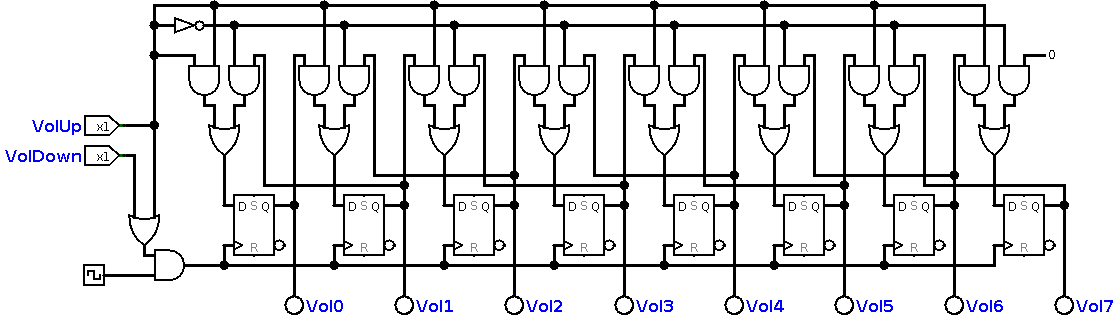
\includegraphics[scale=0.372]{images/stagetwo.png}
    \caption{Circuit used for stage two -- Volume control}
\end{figure}
For this stage I assumed that the pins/buttons could continuously make the volume go
up or down. With this in mind, I found it to be most appropriate to use a bi-directional
shift register to control volume values. This is for two reasons:

\begin{itemize}
    \item It allows for easy raising or lowering of the required bar graph display
    \item It inherently does not allow for overflowing or underflowing values
\end{itemize}

Of course, this isn't just a bi-directional shift register. I've made some modifications to
the inputs of circuit so that it may fit our application better. There are two inputs to
this ciruit: the volume up and volume down pins. Both of these pins are connected to an
or gate which feeds into an and gate that also has the clock as the input. This allows us
to control when we allow the clock pulse to feed into the circuit so that it can hold state
and not cause any unexpected behaviour.

\bigskip

This design is not without flaws however, since if you put both inputs on then it will simply
continue increasing the volume. I did attempt to fix this by replacing the or gate with a
xor gate, but this had it's own issue. When the xor gate was in use, occasionally when you go
from having both inputs on to just having the volume down input on it would go all the way to
zero from any state, which is not behaviour that we want. This may be solvable with a latch
to time the inputs to the clock, but I haven't been able to apply this yet. As such, I chose
the solution that gives the most consistent and useful output to the user.

\pagebreak

\section*{Stage 3}
\begin{figure}[h]
    \centering
    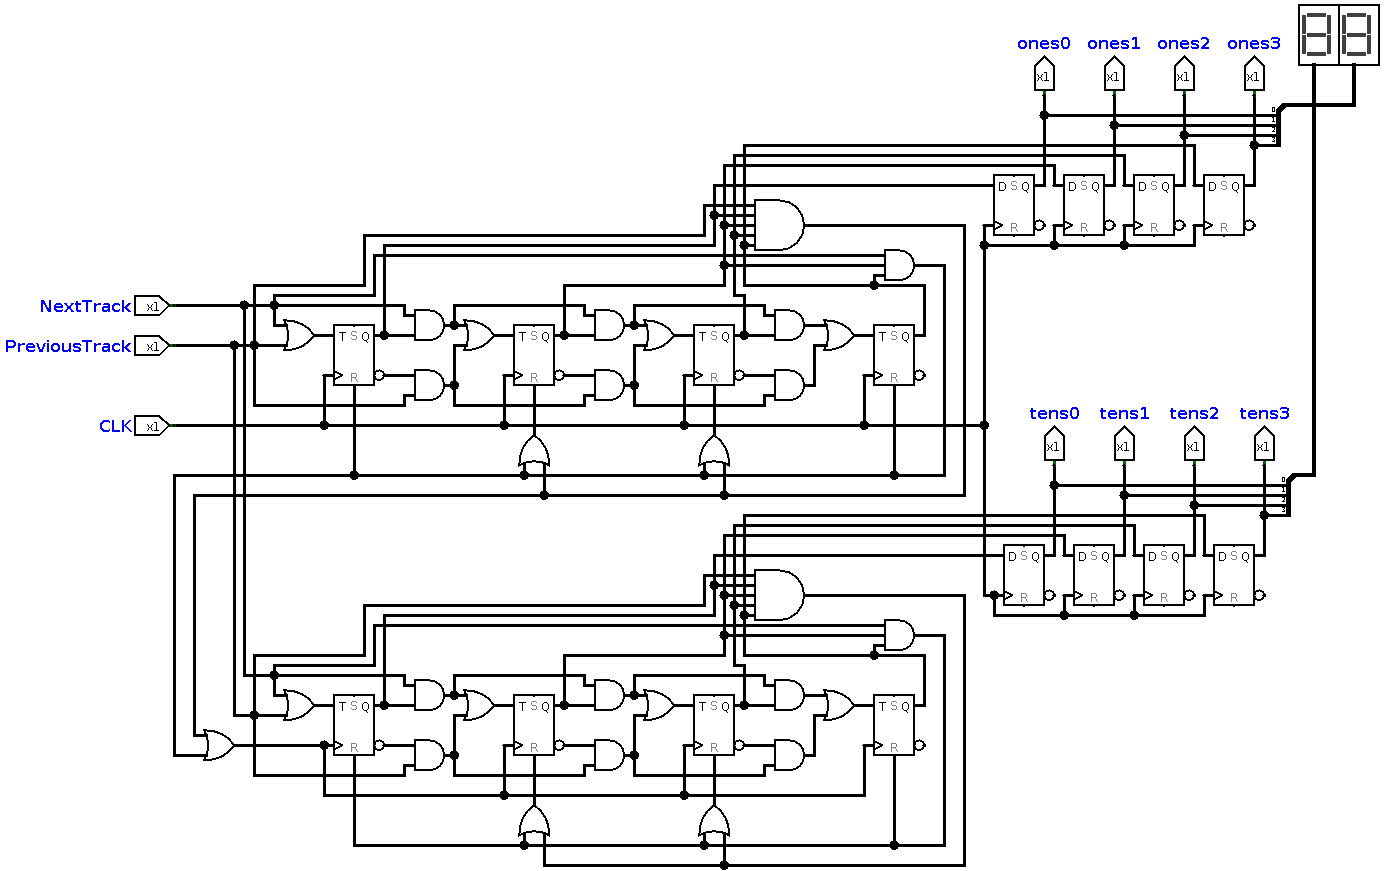
\includegraphics[scale=0.3]{images/stagethree.png}
    \caption{Circuit used for stage three -- Track control}
\end{figure}
Here we have the track control circuit that can be interacted with by using two buttons. For
this I assumed that for inputs we can have buttons that continuously increment or decrement the
track number. This circuit, unlike the previous two, are what I like to refer to as "semi
synchronous" since while half of it is synched to a common clock, the other half is actually
aysynchronously clocked to the output of the first half.

\bigskip

The basic overview is that this circuit works by having two 4 bit mod 10 bi-directional
counters, one for the units column and one for the tens column of our decimal number that is
being displayed on two hex displays. For both counters there is logic to allow it to count
forwards or backwards in the form of two and gates and an or gate for each T flip flop. As well
as this, there are two and gates that are used to check for a state of 10 (little endian 0101) and
15 (little endian 1111) so that it can wrap around to the correct numbers. For each and gate there
is also a control bit which is controlled by the next and previous button respectively to ensure
that they are only "active" as long as they need to be for checking states. This makes sure that
we're not getting false positive states when going either direction, allowing for smooth operation.

\bigskip

For each circuit however, there are very slight differences. The main thing of note is that it the
second counter is not connected to the common clock for the circuit. This is because the first
counter will instead feed the signal from overflow or underflow states (when it hits 10 or 15
respectively) into the clock input of the next counter. This is why I mentioned previously that
this circuit is "semi synchronous". However, this does not end up mattering all too much since
there is a fully clocked register that is used as a buffer to ensure that all output signals are
clean and no illegal states get out.

\bigskip

There is one issue with this circuit, that being that the registers delay the output signals by a
tick. This is a worthwhile trade off in my opinion however, since this ensures data integrity which
is important for preventing unexpected behaviour caused by illegal states.

\section*{Stage 4 and 5}
\begin{figure}[h]
    \centering
    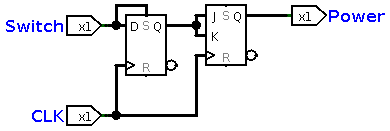
\includegraphics[scale=0.5]{images/stagefour.png}
    \caption{Circuit used for stage four -- Turning on and off}
\end{figure}
Both of these stages go hand in hand for the most part since they work off each other.
The circuit above is what I consider to be the "master" control circuit for handling
the on/off state of the entire music player. The reason for this is because the input from
the user only needs to go into one place, and from here the "on" signal can propogate out
to the rest of the circuits, decreasing the overall complexity of the circuit while also
allowing for easier expandibility elsewhere in the circuit. Take the following circuit
for the play/pause functionality for example:
\begin{figure}[h]
    \centering
    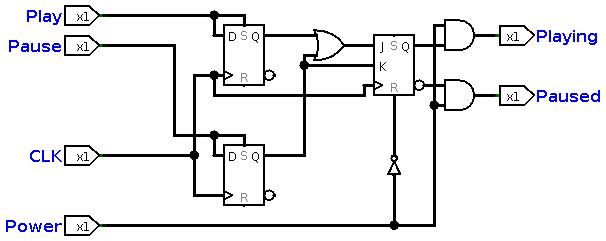
\includegraphics[scale=0.5]{images/stageonenew.png}
    \caption{Stage one circuit modified to work with on/off functionality}
\end{figure}

\pagebreak

In this modified circuit for stage one, we have added a "power" pin that acts as a signal
to tell this circuit if it should be on or off. If it is off then we turn off the control
bits for the output off so no output is sent and we reset the JK flip flop so that when
it's turned back on it will be in the paused state. The master control circuit's output
then feeds into this power input to provide that signal. Having that logic in the master
circuit means that we only need to have one JK flip flop handling every circuit's power
state instead of requiring one for every circuit.

\bigskip

Along with this, the state for each circuit is stored internally within the flip flops
that already exist. Outputs for these circuits are just disabled when the power pin is
low, and once the power pin is high outputs are enabled again and the previous state is
restored to the user's outputs. The reason I approached stage 5 like this is for two
reasons:
\begin{itemize}
    \item To not over-complicate what is already a complicated set of circuits
    \item To re-use what we already have, but in a different capacity
\end{itemize}
This gives our circuit an overall smaller footprint while still maintaining the same
functionality to the user.
\begin{figure}[h]
    \centering
    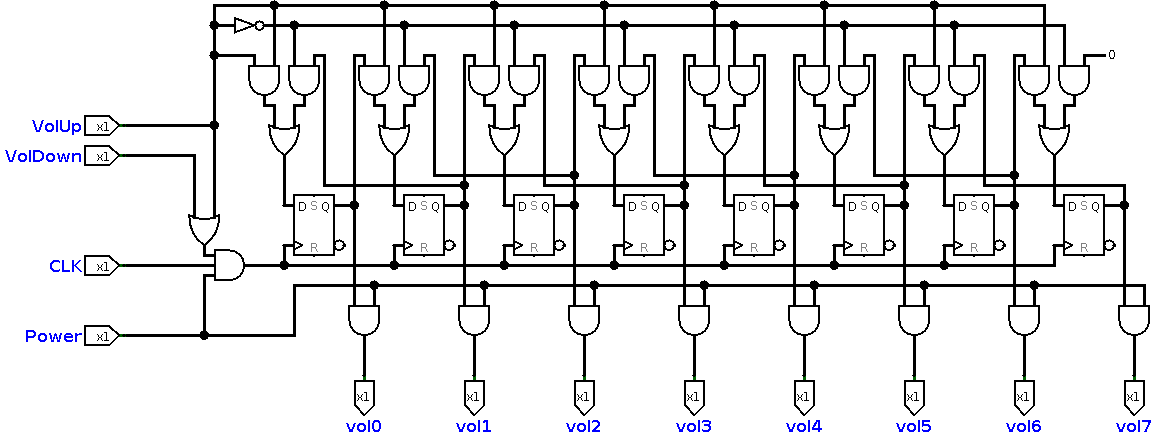
\includegraphics[scale=0.35]{images/stagetwonew.png}
    \caption{Stage two circuit modified to work with on/off functionality}
\end{figure}
\begin{figure}[h]
    \centering
    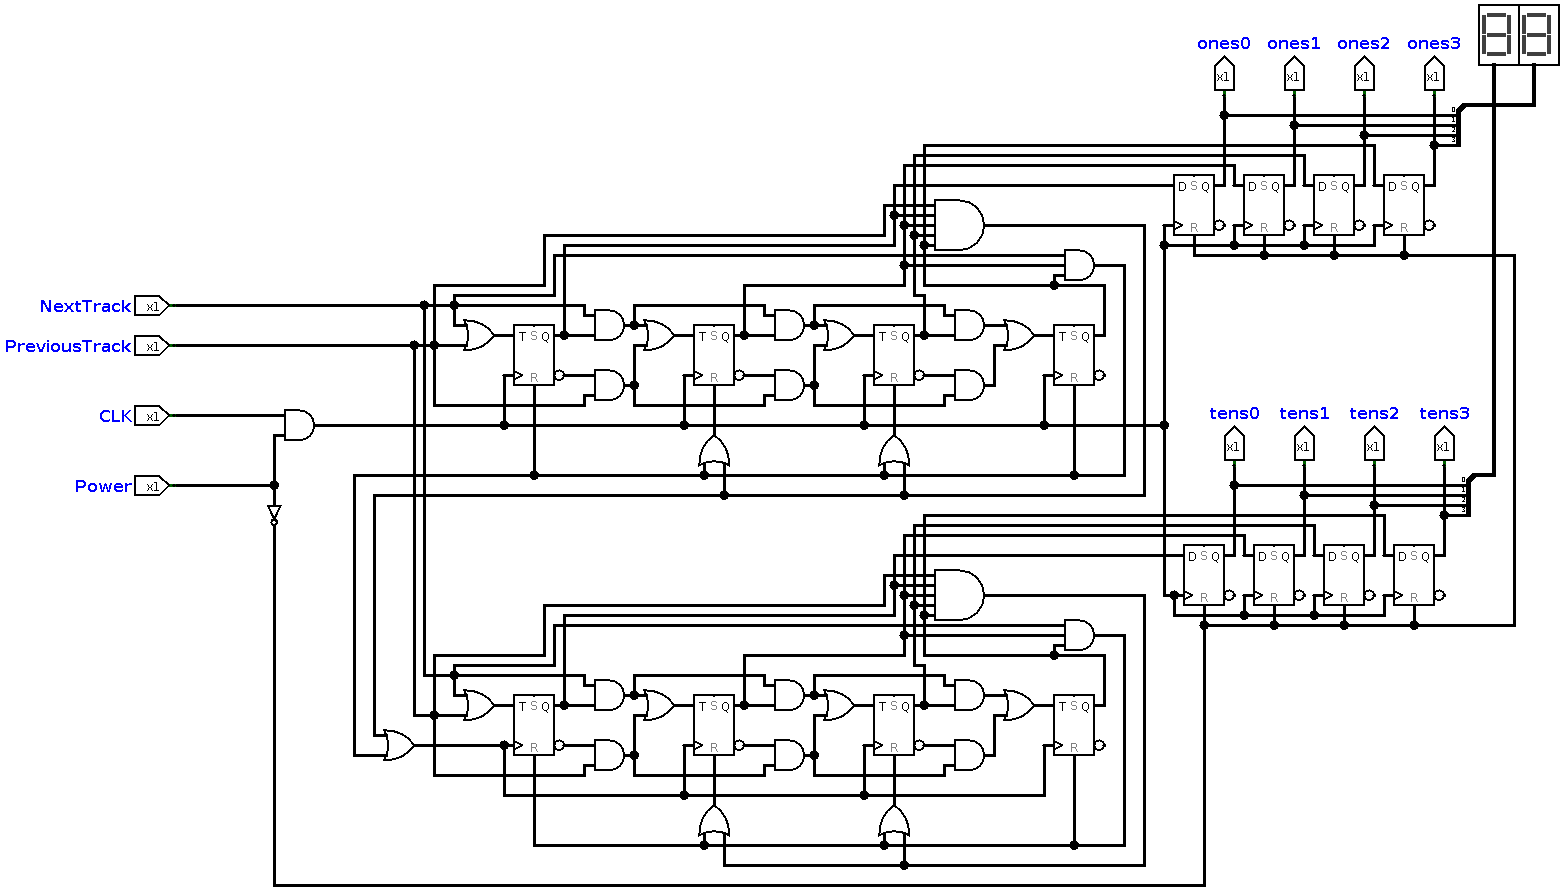
\includegraphics[scale=0.25]{images/stagethreenew.png}
    \caption{Stage three circuit modified to work with on/off functionality}
\end{figure}

\pagebreak

\section*{Bonus Stage}
\begin{figure}[h]
    \centering
    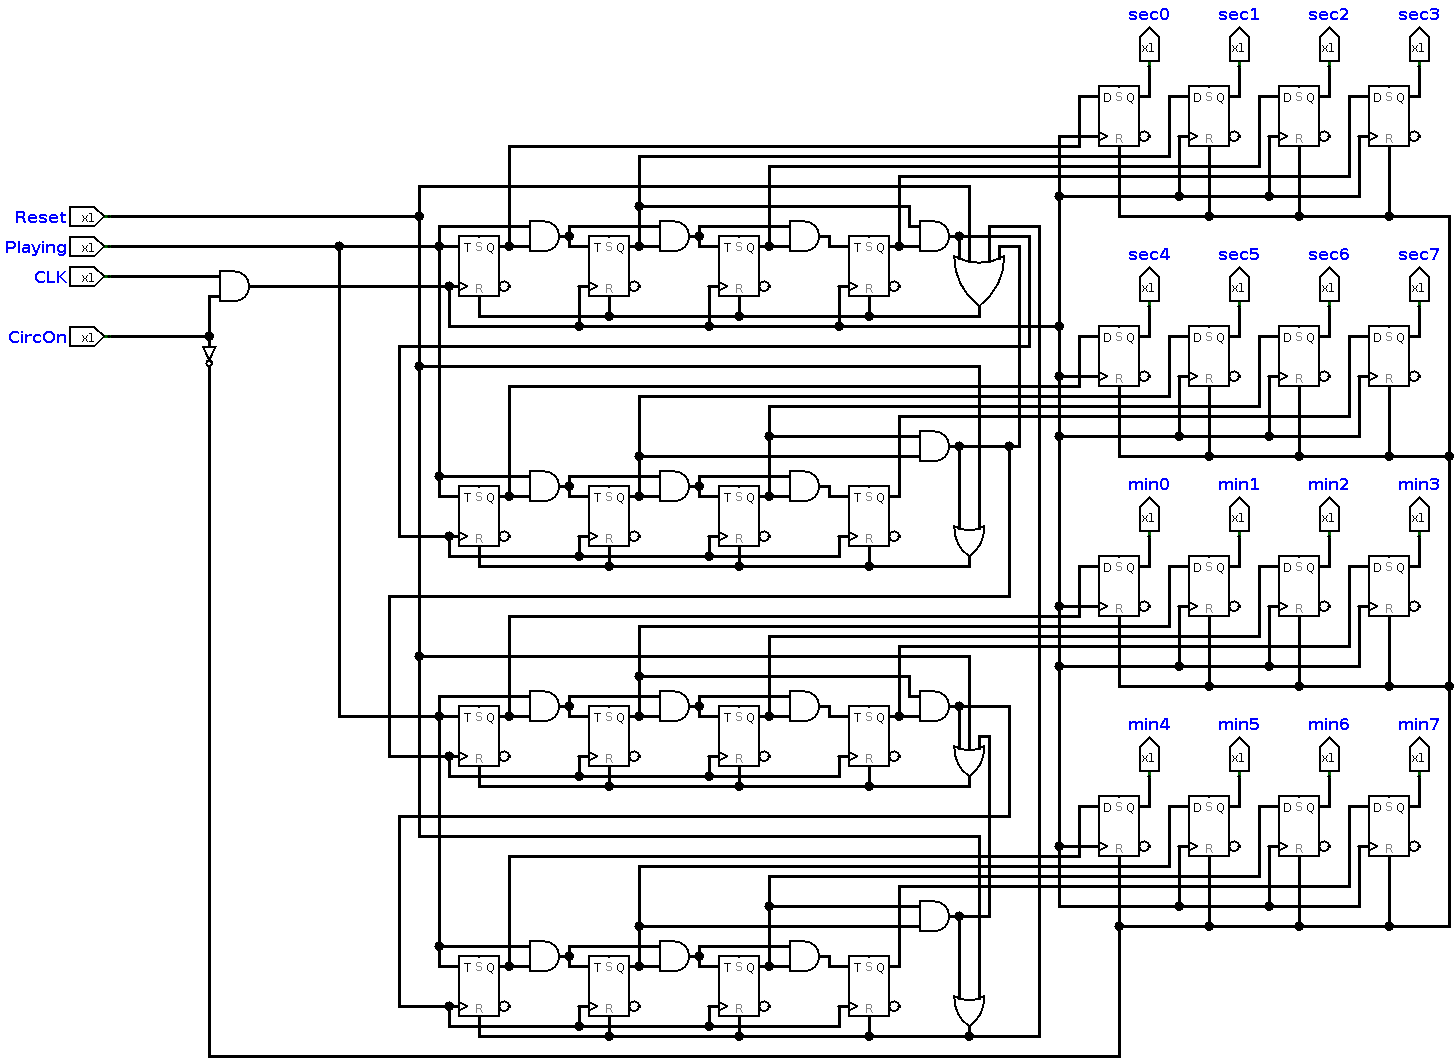
\includegraphics[scale=0.25]{images/bonusstage.png}
    \caption{Circuit used for the bonus stage -- Track timer}
\end{figure}
I have also attempted the bonus stage in this assignment, which with the previous circuits
that have been done is actually fairly trivial. This is mostly just a a reworked circuit
from stage 3, using the same counter design (however only uni-directional this time)
and the same concept for making the counter MOD 10. There are a number of changes however:
\begin{itemize}
    \item There are now four counters total (two for the minutes and two for the seconds)
    \item Each group of two counters is collectively MOD 60
    \item The entire counter goes from 0 minutes and 0 seconds to 59 minutes and 59 seconds
    \item The counter only counts in one direction
    \item The counter must also be able to be reset by a single pin
\end{itemize}
Most of these changes were trivial, requiring only small modifications of logic or a small
amount of new wiring for any of the new features. As a result, almost everything relevant
to the circuit in stage 3 is also the case in this circuit.

\pagebreak

\section*{Final Circuit}
For the final circuit I have abstracted away all of the stages into their own circuits as
to make the final circuit where we have everything together more compact and easy to
understand. Here there are all of the pieces brought together and their inputs are
implemented along with outputs appropriate to each circuit. Generally speaking, there
are some unresolved issues with some of the circuits:
\begin{itemize}
    \item Setting the clock speed higher than roughly 4Hz can have unexpected behaviour on some inputs
    \item Circuits that use the button latch circuit (stages 1 and 4) may toggle back to it's previous state occasionally
\end{itemize}
\begin{figure}[h]
    \centering
    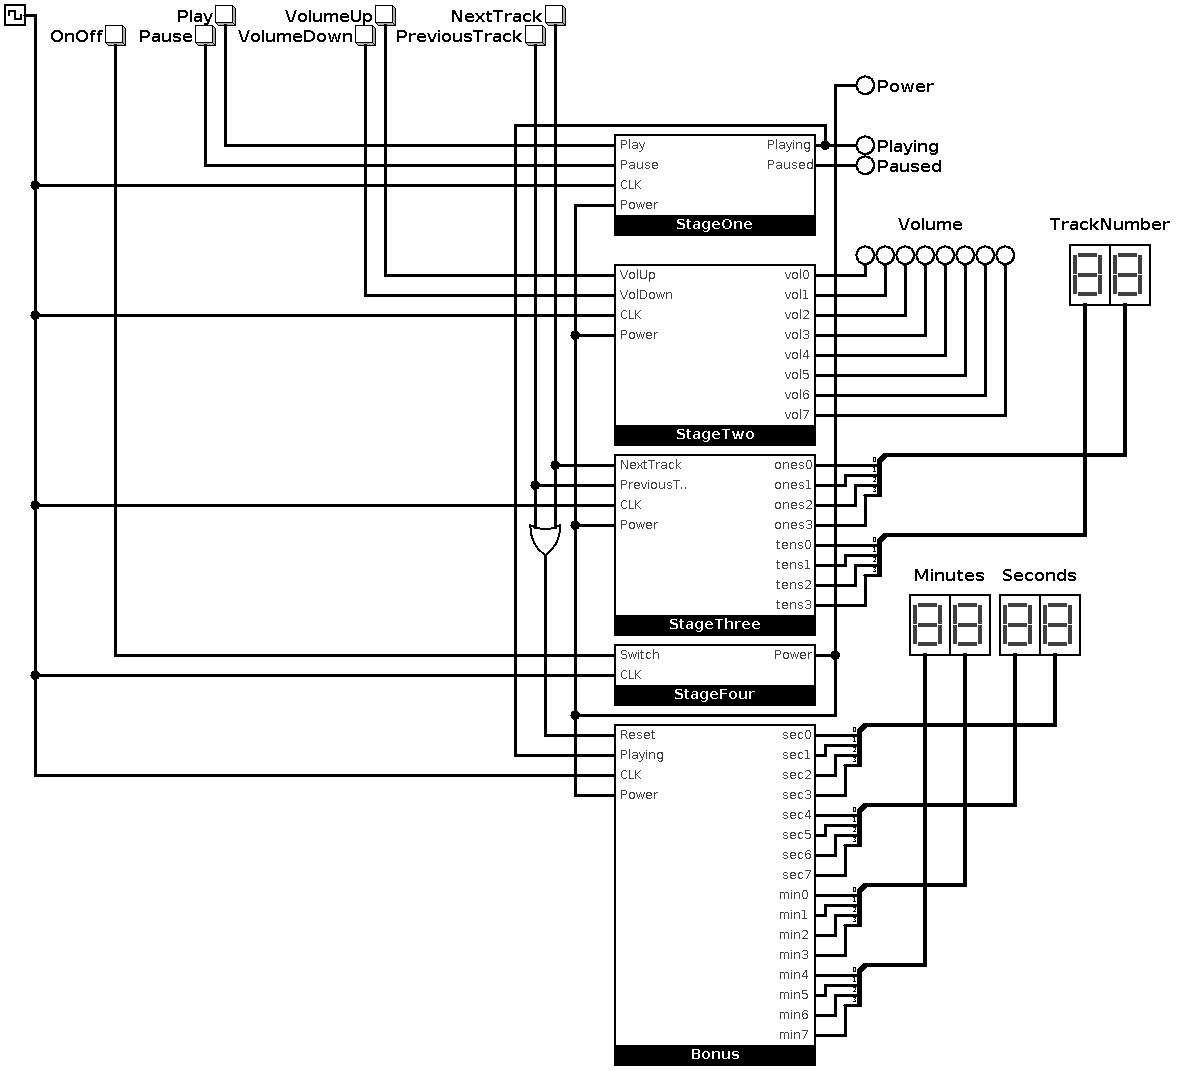
\includegraphics[scale=0.35]{images/main.png}
    \caption{The final circuit with all stages together}
\end{figure}

\end{document}
